\documentclass[]{article}
%\usepackage{ctex,hyperref}% 输出汉字
\usepackage{amsmath,amssymb,amsfonts}
\usepackage{amsthm,amsmath,amssymb}
\usepackage{mathrsfs}
%opening
\usepackage{setspace}
\usepackage{lipsum}
\usepackage{graphicx}% 图片插入宏包
\usepackage{subfigure}% 并排子图
\usepackage{float}% 浮动环境,用于调整图片位置
\usepackage[export]{adjustbox}% 防止过宽的图片
\usepackage{amsmath}
\usepackage{extarrows}
\graphicspath{{Figures/}}%文章所用图片在当前目录下的 Figures目录
\title{Space-Fixed and Body-Fixed Frames}
\author{Yun-ting Bu}

\begin{document}
	
	\maketitle
\section{Coordinate Rotations and Angular Momentum}

If the physical system in space $(X,Y,Z)$ is rotated by an infinitesimal angle $\epsilon$ along the dirction of a unit vector $\mathbf{\hat{u}}$ to a new point in space $(X^\prime,Y^\prime,Z^\prime)$, then a vector $\mathbf{A}$ is transformed to the new one via the relation
\begin{align}
	\mathbf{A^\prime}&=R_u(\epsilon)\mathbf{A}\nonumber\\
	&=\mathbf{A}-\epsilon(\mathbf{\hat{u}}\times\mathbf{A})
	\label{d1}
\end{align}
In particular, the coordinate vector $\mathbf{r}$ also transforms by this relation.\par 
When the physical sysytem is rotated from the point $\mathbf{r}$ to the new point $\mathbf{r^\prime}$ in space, the value of the old function at $\mathbf{r}$ must be the same as the new function at $\mathbf{r^\prime}$ or
\begin{equation}
	\psi^\prime(\mathbf{r^\prime})=\psi(\mathbf{r})
\end{equation}
If we define a rotation operator $R$ for the transformation of the function by 
\begin{equation}
	\psi^\prime(\mathbf{r})=R\psi(\mathbf{r})
\end{equation}
then we have the relation
\begin{equation}
	R\psi(\mathbf{r^\prime})=\psi(\mathbf{r})=\psi[R^{-1}_u(\epsilon)\mathbf{r^\prime}]
\end{equation}
	By using \eqref{d1} for the coordinate vector $\mathbf{r}$, we obtain
\begin{align}
	R\psi(\mathbf{r^\prime})&=\psi[\mathbf{r^\prime}-\epsilon(\mathbf{\hat{u}}\times\mathbf{r^\prime})]\nonumber\\
	&=\sum\limits_{n=0}^\infty\dfrac{[-\epsilon(\mathbf{\hat{u}}\times\mathbf{r^\prime})\cdot\nabla]^n}{n!}\psi(\mathbf{r^\prime})\nonumber\\
	&=\sum\limits_{n=0}^\infty\dfrac{(-\mathrm{i}/\hbar\epsilon\mathbf{\hat{u}}\cdot\mathbf{J})^n}{n!}\psi(\mathbf{r^\prime})
\end{align}
where $\mathbf{J}=-\mathrm{i}\hbar\mathbf{r}\times\nabla$ is yhe angular momenyum operator. By replacing $\mathbf{r^\prime}$ by $\mathbf{r}$, we arrive at the transformation relation
\begin{align}
	\psi^\prime(\mathbf{r})&=R\psi(\mathbf{r})\nonumber\\
	&=\mathrm{exp}\left( -\dfrac{\mathrm{i}}{\hbar}\epsilon J_u\right) \psi(\mathbf{r})
\end{align}
\section{Rotation Matrix}
\subsection{Definition}

Let $(X,Y,Z)$ denote the space-fixed(SF) coordinate system and $(x,y,z)$ denote the rotated (body-fixed or molecular) coordinate system which is obtained throught rotation of the SF coordinate system by the three Euler angles as shown in Fig.\eqref{Figure 1}. 
\begin{figure}[H]
	\centering
	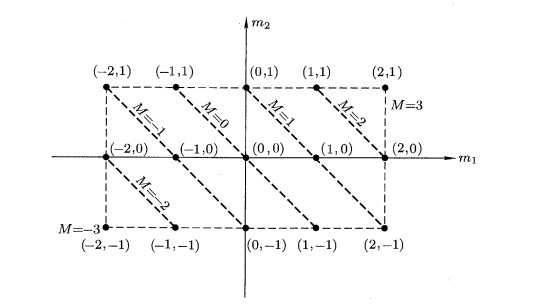
\includegraphics[scale=0.2]{1.png}
	\caption{SF $(X,Y,Z)$ and BF $(x,y,z)$ coordinate systems specified by three Euler angles $(\phi,\theta,\chi)$. $Y^\prime$ is the $Y-$axis of the intermediate coordinate system.}
	\label{Figure 1}
\end{figure}

The rotation of the physical system from the SF $\rightarrow$ BF frame can be represented by the product of three successive rotations
\begin{equation}
	\mathbf{R}(\phi,\theta,\chi)=\mathrm{e}^{-\mathrm{i}\chi J_z}\mathrm{e}^{-\mathrm{i}\theta J_{Y^\prime}}\mathrm{e}^{-\mathrm{i}\phi J_Z}
	\label{d7}
\end{equation}
where $J_{Y^\prime}$ is the angular momentum along the intermediate $Y^\prime$ axis. Using the transformation relation for operators under unitary transformation, we can write
\begin{equation}
	\mathrm{e}^{-\mathrm{i}\chi J_z}=\mathrm{e}^{-\mathrm{i}\theta J_{Y^\prime}}\mathrm{e}^{-\mathrm{i}\chi J_Z}\mathrm{e}^{-\mathrm{i}\theta J_{Y^\prime}}
\end{equation}
and 
\begin{equation}
	\mathrm{e}^{-\mathrm{i}\theta J_{Y^\prime}}=\mathrm{e}^{-\mathrm{i}\phi J_Z}\mathrm{e}^{-\mathrm{i}\phi J_Z}\mathrm{e}^{-\mathrm{i}\phi J_Z}
\end{equation}
By applying the above equations, we can rewrite the rotation matrix in \eqref{d7} as
\begin{equation}
	\mathbf{R}(\phi,\theta,\chi)=\mathrm{e}^{-\mathrm{i}\phi J_Z}\mathrm{e}^{-\mathrm{i}\theta J_Y}\mathrm{e}^{-\mathrm{i}\chi J_Z}
	\label{d10}
\end{equation}
where $J_Y$ and $J_Z$ are angular momentum projections on the $Y$ and $Z$ axes in the SF coordinate system. \eqref{d10} states that the rotation operation depicted in Fig.\ref{Figure 1} can be equally achieved by three successive rotations defined in the same coordinate system but with a reversal of the order of relation.\par 
Upon rotation, the new state vector $|\psi\rangle^\prime$ is related to old one $|\psi\rangle$ through a unitary transformation
\begin{equation}
	|\psi\rangle^\prime=\mathbf{R}(\phi,\theta,\chi)|\psi\rangle
\end{equation}
If $|\psi\rangle$ is an angular momentum eigenstate $| JM\rangle$, we then have
\begin{align}
	|JM\rangle^\prime&=\sum\limits_{M^\prime}|JM^\prime\rangle\langle JM^\prime|\mathbf{R}(\phi,\theta,\chi)|JM\rangle\nonumber\\
	&=\sum\limits_{M^\prime}|JM^\prime\rangle D^J_{M^\prime M}(\phi,\theta,\chi)
\end{align}
where the rotation matrix is defined as 
\begin{align}
	D^J_{M^\prime M}(\phi,\theta,\chi)&=\langle JM^\prime|\mathbf{R}(\phi,\theta,\chi)|JM\rangle\nonumber\\
	&=\mathrm{e}^{-\mathrm{i}\phi M^\prime}d^J_{M^\prime M}(\theta)\mathrm{e}^{-\mathrm{i}\chi M}
\end{align}
where $d^J_{M^\prime M}(\theta)$ is the reduced rotation matrix and is real. The explicit expression for the reduced rptation matrix is given by Wigner
\begin{align}
	d^J_{M^\prime M}(\theta)=&\sqrt{(J+M^\prime)!(J-M^\prime)!(J+M)!(J-M)!}\nonumber\\
	&\times\sum\limits_\nu\dfrac{(-1)^\nu}{(J-M^\prime-\nu)!(J+M-\nu)!(\nu+M^\prime-M)!\nu!}\nonumber\\
	&\times\left( \mathrm{cos}\left( \dfrac{\theta}{2}\right) \right) ^{2J+M-M^\prime-2\nu}\left( -\mathrm{sin}\left( \dfrac{\theta}{2}\right) \right) ^{M^\prime-M+2\nu}
\end{align}
where the sum over $\nu$ is for all integers for which yhe factorial arguments are nonnegative.
\subsection{Special Properties}
The rotation matrix $d^J_{M^\prime M}(\theta)$ has the following symmetry properties:
\begin{equation}
	d^J_{M^\prime M}(\theta)=d^J_{-M-M^\prime}(\theta)
\end{equation}

\begin{equation}
	d^J_{M^\prime M}(-\theta)=d^J_{MM^\prime}(\theta)=(-1)^{M^\prime-M}d^J_{M^\prime M}(\theta)
\end{equation}
In the case of $M^\prime=0$, $d^J_{MM^\prime}(\theta)$ is related to the associated Legendre polynomial
\begin{equation}
	d^J_{M0}(\theta)=(-1)^M\sqrt{\dfrac{(L-M)!}{(L+M)!}}\mathrm{P}_{JM}(\mathrm{cos}\theta)
\end{equation}
\subsection{Orthogonality}
The rotation matrix $D^J_{M^\prime M}$ is orthogonal
\begin{align}
	\langle D^{J^\prime}_{M^\prime N^\prime}|D^J_{MN}\rangle&=\int_0^{2\pi}\mathrm{d}\phi\int_0^\pi\mathrm{sin}\theta\mathrm{d}\theta\int_0^{2\pi}\mathrm{d}\chi D^{J^\prime*}_{M^\prime N^\prime}(\phi,\theta,\chi)D^J_{MN}(\phi,\theta,\chi)\nonumber\\
	&=\dfrac{8\pi^2}{2J+1}\delta_{J^\prime J}\delta_{M^\prime M}\delta_{N^\prime N}
\end{align}
Since the rotation operator is unitary, the inverse of the rotation matrix is given by its hermitian adjoint
\begin{equation}
	[D^J]^{-1}_{MM^\prime}=D^{J*}_{M^\prime M}
\end{equation}
\section{Transformation Between SF and BF Basis}
If the total angular momentum of a molecular system $\mathbf{J}$ is the sum of two independent angular momenta $\mathbf{j}$ and $\mathbf{l}$($\mathbf{l}$ is usually the orbital angular momentum), the SF angular momentum eigenstate in the coupled representation $|JMjl\rangle$ is obtained through the orthogonal transformation from the uncoupled representation 
\begin{equation}
	|JMjl\rangle =\sum\limits_m\langle jmlM-m|JM\rangle|jm\rangle|lM-m\rangle
\end{equation}
which can also be reversed to yield
\begin{equation}
	|jm\rangle|lM-m\rangle=\sum\limits_J\langle jmlM-m|JM\rangle|JMjl\rangle
\end{equation}
where the summation includes all allowed values of $m$ or $J$. It is easy to verify that the SF eigenfunction $\mathrm{Y}^{JM}_{jl}$ is also an eigenfunction of the parity 
\begin{equation}
	\hat{p}\mathrm{Y}^{JM}_{jl}(\mathbf{\hat{R}},\mathbf{\hat{r}})=\mathrm{Y}^{JM}_{jl}(\mathbf{-\hat{R}},-\mathbf{\hat{r}})=p\mathrm{Y}^{JM}_{jl}(\mathbf{\hat{R}},\mathbf{\hat{r}})
\end{equation}
with the parity $p$ given by
\begin{equation}
	p=(-1)^{j+l}
	\label{d23}
\end{equation}
In the SF coordinate system, the total angular momentum eigenfunction can be written explicitly
\begin{equation}
	\mathrm{Y}^{JM}_{jl}(\mathbf{\hat{R}},\mathbf{\hat{r}})=\sum\limits_m\langle jmlM-m|JM\rangle\mathrm{Y}^m_j(\hat{r})\mathrm{Y}^{M-m}_l(\hat{R})
\end{equation}
where the unit vectors denote spatial orientation $\mathbf{\hat{R}}=(\theta_R,\phi_R)$ and $\mathbf{\hat{r}}=(\theta_r,\phi_r)$.

If the molecular system is rotated from the SF frame to the BF frame by the three Euler angles $(\phi,\theta,\chi)$ in space, then the rotated angular momentum wavefunction $\mathrm{Y}^{JM}_{jl}$(in the SF frame) is obtained from the unrotated one $\widetilde{\mathrm{Y}}^{JK}_{jl}$ by the transformation relation
\begin{equation}
	\mathrm{Y}^{JM}_{jl}(\mathbf{\hat{R}},\mathbf{\hat{r}})=\sum\limits_KD^J_{KM}(\phi,\theta,\chi)\widetilde{\mathrm{Y}}^{JK}_{jl}(\mathbf{\hat{R}},\mathbf{\hat{r}})
	\label{d25}
\end{equation}
where $\widetilde{\mathrm{Y}}^{JK}_{jl}(\mathbf{\hat{R}},\mathbf{\hat{r}})$ is the unrotated wavefunction of $\mathrm{Y}^{JM}_{jl}(\mathbf{\hat{R}},\mathbf{\hat{r}})$ in the BF frame. If we choose the $z$ axis in the BF frame to coincide with the direction of the unit vector $\hat{R}$, then we have $\hat{R}=(0,0)$ and $\hat{r}=(\gamma,0)$. Thus the unrotated wavefunction simplifies to
\begin{align}
	\widetilde{\mathrm{Y}}^{JK}_{jl}(00,\gamma0)&=\sum\limits_m\langle jmlK-m|JK\rangle\mathrm{Y}^m_j(\gamma,0)\mathrm{Y}^{K-m}_l(00)\nonumber\\
	&=\sqrt{\dfrac{2l+1}{4\pi}}\langle jKl0|JK\rangle \mathrm{Y}^K_j(\gamma,0)
\end{align}
\eqref{d25} can thus be rewritten as
\begin{align}
	\mathrm{Y}^{JM}_{jl}(\mathbf{\hat{R}},\mathbf{\hat{r}})&=\langle\hat{R}\hat{r}|JMjl\rangle\nonumber\\
	&=\sqrt{\dfrac{2l+1}{4\pi}}\sum\limits_K\langle jKl0|JK\rangle D^J_{KM}(\phi,\theta,\chi)\mathrm{Y}^K_j(\gamma,0)
	\label{d27}
\end{align}

We can now define a body-fixed angular momentum function by
\begin{equation}
	\mathcal{Y}^{JM}_{jK}=\widetilde{D}^J_{KM}\mathrm{P}_{jK}
	\label{d28}
\end{equation}
where $\mathrm{P}_{JK}=\sqrt{2\pi}\mathrm{Y}^{K}_j(\gamma,0)$ are normalized associated Legendre polynomials and $\widetilde{D}^J_{KM}$ are normalized rotation matrices defined as
\begin{equation}
	\widetilde{D}^J_{KM}=\sqrt{\dfrac{2J+1}{8\pi^2}}D^J_{KM}
\end{equation}
Using \eqref{d28}, we can rewrite \eqref{d27} as an orthogonal transformation between SF and BF angular momentum function
\begin{equation}
	\mathrm{Y}^{JM}_{jl}=\sum\limits_KC_{lK}\mathcal{Y}^{JM}_{jK}
	\label{d30}
\end{equation} 
where the orthogonal transformation matrix is
\begin{equation}
	C_{lK}=\sqrt{\dfrac{2l+1}{2J+1}}\langle jKl0|JK\rangle
\end{equation}
\eqref{d30} can be inverted to yield
\begin{equation}
	\mathcal{Y}^{JM}_{jK}=\sum\limits_lC_{lK}\mathrm{Y}^{JM}_{jl}
\end{equation}

By performing the parity operation on $\mathcal{Y}^{JM}_{jK}$ we obtain
\begin{align}
	\hat{p}\mathcal{Y}^{JM}_{jK}&=\sum\limits_lC_{lK}\hat{p}\mathrm{Y}^{JM}_{jl}\nonumber\\
	&=\sum\limits_lC_{lK}(-1)^{j+l}\mathrm{Y}^{JM}_{jl}\nonumber\\
	&=(-1)^J\sum\limits_lC_{l-K}\mathrm{Y}^{JM}_{jl}\nonumber\\
	&=(-1)^J\mathcal{Y}^{JM}_{j-K}
\end{align}
where the symmertry relation for the CG coefficient has been used. Thus, the BF function $\mathcal{Y}^{JM}_{jK}$ is not an eigenfunction of parity. It is thus often convenient to group the $K$ and $-K$ terms together to define a parity-adapted BF angular momentum function as
\begin{align}
	\mathcal{Y}^{JMp}_{jK}&=\dfrac{1}{\sqrt{2(1+\delta_{K0})}}[\mathcal{Y}^{JM}_{jK}+\hat{p}\mathcal{Y}^{JM}_{jK}]\nonumber\\
	&=\dfrac{1}{\sqrt{2(1+\delta_{K0})}}[\mathcal{Y}^{JM}_{jK}+(-1)^P\mathcal{Y}^{JM}_{j-K}]
	\label{d34}
\end{align}
where the total paruty $P$ is defined as $P=(-1)^{J+p}$ with parity $p$ given by the definition of \eqref{d23}. We note that for $K=0$, only even total parity exists. With the definition of \eqref{d34}, we only need to deal with quantum numbers $K\geqslant0$.

Using $\mathcal{Y}^{JMp}_{jK}$ as the BF angular momentum eigenfunction, the transformation relation of \eqref{d30} can be rewritten as
\begin{equation}
	\mathrm{Y}^{JM}_{jl}=\sum\limits_{K\geqslant0}C^p_{lK}\mathcal{Y}^{JMp}_{jK}
\end{equation}
where the $C^p_{lK}$ are given by
\begin{align}
	C^p_{lK}&=\sqrt{2-\delta_{K0}}C_{lK}\nonumber\\
	&=\sqrt{2-\delta_{K0}}\sqrt{\dfrac{2l+1}{2J+1}}\langle jKl0|JK\rangle
\end{align}
\section{Total Angular Momentum in the BF Frame}
If $\hat{J}_i(i=x,y,z)$ denote the projections of the total angular momentum $\mathbf{J}$ along the BF axes, they the anomalous commutation relation
\begin{equation}
	[\hat{J}_i,\hat{J}_j]=\hat{J}_i\hat{J}_j-\hat{J}_j\hat{J}_i=\mathrm{i}\sum\limits_k\epsilon_{ijk}\hat{J}_k
	\label{d39}
\end{equation}
where $\epsilon_{ijk}$ is the standard antisymmetric tensor. As a result of this, the raising and lowering operators of the total angular momentum $\hat{J}_\pm=\hat{J}_x\pm\mathrm{i}\hat{J}_y$ in the BF frame behave like the lowering and raising operators $\hat{J}_\mp=\hat{J}_X\mp\mathrm{i}\hat{J}_Y$ in the SP frame. The following is a formal proof of \eqref{d39} by Van Vleck using direction cosine vectors.\par 
Let $\mathbf{u}^\alpha(\alpha=x,y,z)$ and $\mathbf{e}_i(i=X,Y,Z)$ be unit vectors along the BF axes and SP axes, repectively. Their projections on the SP axis $\mathbf{u}^\alpha_i=\mathbf{u}^\alpha\cdot\mathbf{e}_i$ are called direction cosines. The vectors $\mathbf{u}^\alpha$ obey the vector multiplication rule
\begin{equation}
	\sum\limits_{\alpha\beta}=\epsilon_{\alpha\beta\gamma}\mathbf{u}^\alpha\mathbf{u}^\beta=\mathbf{u}^\gamma 
	\label{d40}
\end{equation}
By the definition of a vector, the commutation relation of $\mathbf{u}^\alpha$ with the total angular momentum $\mathbf{J}$ (space-fixed) is given by
\begin{equation}
	[\hat{J}_i,u^\alpha_j] =\mathrm{i}\sum\limits_k\epsilon_{ijk}u^\alpha_k 
	\label{d41}
\end{equation}
Using \eqref{d40} and \eqref{d41} along with the standard commutation relation of $\mathbf{J}$, it is not difficult to slow that the BF angular momentum $\hat{J}_\alpha=\mathbf{u}^\alpha\cdot\mathbf{J}=\sum_iu^\alpha_i\hat{J}_i$ satisfies the anomalous commutation relation \eqref{d39}.\par 
It should be emphasized here that it is the total angular momentum whoes projection onto the BF representation satisfies the anomalous commulation relation. However, the component angular momenta still satisfy the normal commutation relation. The effect of this anomalous commutation relation $J_\pm$ in the BF frame on BF angular momentum eigenfunctions. The simplest approach is to represent the total angular momentum operator in the BF coordinate system in terms of the three Euler angles and to explicitly work out the following relation
\begin{align}
	\hat{J}_\pm D^J_{KM}&=\sqrt{J(J+1)-K(K\mp1)}D^J_{K\mp 1M}\nonumber\\
	&=\lambda^\mp_{JK}D^J_{K\mp 1M}
\end{align} 
or use the normalized rotation matrix
\begin{equation}
	\hat{J}_\pm\widetilde{D}^J_{KM}=\lambda^\mp_{JK}\widetilde{D}^J_{K\mp1M}
\end{equation}
This is an important relation that has been used to derive the coupling terms of the centrifugal potential for molecular Hamiltonian matrices and a number of other places. For example, we can evaluate the following expression in the BF coordinate system
\begin{align}
	\hat{J}_\pm\hat{\jmath}_\mp\mathcal{Y}^{JM}_{jK}&=(\hat{J}_\pm\widetilde{D}^J_{KM})(\hat{\jmath}_\mp\mathrm{P}_{jK})\nonumber\\
	&=(\lambda^\mp_{JK}\widetilde{D}^J_{K\mp1M})(\lambda^\mp_{jK}\mathrm{P}_{jK\mp1})\nonumber\\
	&=\lambda^\mp_{JK}\lambda^\mp_{jK}\mathcal{Y}^{JM}_{jK\mp1}
\end{align}

The action of the angular momentum operator in the BF frame on parity-adapted BF angular momentum functions yields
\begin{align}
	\hat{J}_z\hat{\jmath}_z\mathcal{Y}^{JMp}_{jK}&=	\hat{J}_z\dfrac{\hbar K}{\sqrt{2(1+\delta_{K0})}}[\mathcal{Y}^{JM}_{jK}-(-1)^P\mathcal{Y}^{JM}_{j-K}]\nonumber\\
	&=\dfrac{\hbar^2 K^2}{\sqrt{2(1+\delta_{K0})}}[\mathcal{Y}^{JM}_{jK}+(-1)^P\mathcal{Y}^{JM}_{j-K}]\nonumber\\
	&=\hbar^2K^2\mathcal{Y}^{JMp}_{jK}
	\label{d45}
\end{align}
and
\begin{align}
	\hat{J}_\pm\hat{\jmath}_\mp\mathcal{Y}^{JMp}_{jK}=&\dfrac{1}{\sqrt{2(1+\delta_{K0})}}\left[ \lambda^\mp_{JK}\lambda^\mp_{jK}\mathcal{Y}^{JM}_{jK\mp1}\right. \nonumber\\
	&\left. +(-1)^P\lambda^\pm_{JK}\lambda^\pm_{jK}\mathcal{Y}^{JM}_{j-K\mp1}\right] 
	\label{d46}
\end{align}
\subsection{Matrix Elements of the $\mathbf{L}^2$ operator in the BF Basis}
Using result derived in the preceding section for angular momentum operators in the BF frame, we can derive the matrix elements of the orbital angular momentum $\mathbf{L}^2$ in BF basis that are needed to construct the matrix elements of the centrifugal potential. Using the parity-adapted BF angular momentum basis, the matrix elements in question are defined by
\begin{equation}
	W^{JMpj}_{K^\prime K}=\langle \mathcal{Y}^{JMp}_{jK^\prime}|\mathbf{L}^2|\mathcal{Y}^{JMp}_{jK}\rangle
	\label{d47}
\end{equation}
where the parity-adapted BF angular momentum basis $\mathcal{Y}^{JMp}_{jK}$ is defined in \eqref{d34}.\par 
To begin the derivation, we first write the orbital angular momentum operators as
\begin{equation}
	\mathbf{L}^2=\mathbf{J}^2-\mathbf{j}^2=(J^2+j^2-2\hat{J}_z\hat{\jmath}_z)-(\hat{J}_+\hat{\jmath}_-+\hat{J}_-\hat{\jmath}_+)
\end{equation}
where $\mathbf{J}$ and $\mathbf{j}$ are, respectively, the total and internal angular momentum operators. Since $\mathbf{L}^2$ is a scalar operator, it is invariant with respect to the reference frame in which the angular momentum operators are projected. Thus we can project the angular momentum operators $\mathbf{J}$ and $\mathbf{j}$ in the BF frame and keep in mind that the total angular momentum operator $\mathbf{J}$ satisfies the anomalous commutation relation. Using the result of  \eqref{d45}, the matrix element in \eqref{d47} is then written as
\begin{align}
	W^{JMpj}_{K^\prime K}=&[J(J+1)+j(j+1)-2K^2]\delta_{K^\prime K}\nonumber\\
	&-\langle \mathcal{Y}^{JMp}_{jK^\prime}|\hat{J}_+\hat{\jmath}_-+\hat{J}_-\hat{\jmath}_+|\mathcal{Y}^{JMp}_{jK}\rangle
	\label{d49}
\end{align}

The matrix element in the second bracket in \eqref{d49} can be calculated as follows. First, we use the result of \eqref{d46} to write
\begin{align}
	(\hat{J}_+\hat{\jmath}_-+\hat{J}_-\hat{\jmath}_+)\mathcal{Y}^{JMp}_{jK}=&\dfrac{1}{\sqrt{2(1+\delta_{K0})}}\left\lbrace \lambda^+_{JK}\lambda^+_{jK}[\mathrm{Y}^{JM}_{jK+1}+(-1)^P\mathrm{Y}^{JM}_{j-K-1}]\right. \nonumber\\
	&\left.+\lambda^-_{JK}\lambda^-_{jK}[\mathrm{Y}^{JM}_{jK-1}+(-1)^P\mathrm{Y}^{JM}_{j-K+1}]\right\rbrace 
\end{align} 
Since $K\geqslant0$, we can separate the $K=0$ case from the second bracket in the preceding equation and use definition \eqref{d34} to rewrite the equation
\begin{align}
	(\hat{J}_+\hat{\jmath}_-+\hat{J}_-\hat{\jmath}_+)\mathcal{Y}^{JMp}_{jK}&=\lambda^+_{JK}\lambda^+_{jK}\dfrac{1}{\sqrt{1+\delta_{K0}}}\mathcal{Y}^{JMp}_{jK+1}+\lambda^-_{JK}\lambda^-_{jK}\dfrac{\delta_{K0}}{\sqrt{1+\delta_{K0}}}\nonumber\\
	&\quad\times\mathcal{Y}^{JMp}_{jK+1}+\lambda^-_{JK}\lambda^-_{jK}(1-\delta_{K0})\sqrt{\dfrac{1+\delta_{K-1,0}}{1+\delta_{K0}}}\mathcal{Y}^{JMp}_{jK-1}\nonumber\\
	&=\lambda^+_{JK}\lambda^+_{jK}\sqrt{1+\delta_{K0}}\mathcal{Y}^{JMp}_{jK+1}+\lambda^-_{JK}\lambda^-_{jK}(1-\delta_{K0})\nonumber\\
	&\quad\times\sqrt{1+\delta_{K1}}\mathcal{Y}^{JMp}_{jK-1}
\end{align}
Thus we have determined the matrix element in \eqref{d47} to be
\begin{align}
	W^{JMpj}_{K^\prime K}=&[J(J+1)+j(j+1)-2K^2]\delta_{K^\prime K}-\lambda^+_{JK}\lambda^+_{jK}\sqrt{1+\delta_{K0}}\delta_{K^\prime K+1}\nonumber\\
	&-\lambda^-_{JK}\lambda^-_{jK}\sqrt{1+\delta_{K1}}\delta_{K^\prime K-1}
	\label{d52}
\end{align}

One could also calculate the matrix element of \eqref{d47} by transforming the BF basis to the SF basis. We can calculate the matrix element by
\begin{align}
	W^{JMpj}_{K^\prime K}&=\sum\limits_{ll^\prime(p)}C^p_{l^\prime K^\prime}C^p_{lK}\langle \mathrm{Y}^{JM}_{jl^\prime}|\mathbf{L}^2|\mathrm{Y}^{JM}_{jl}\rangle\nonumber\\
	&=\sum\limits_{ll^\prime(p)}l(l+1)C^p_{l^\prime K^\prime}C^p_{lK}\nonumber\\
	&=\sum\limits_{ll^\prime(p)}\sqrt{2-\delta_{K^\prime0}}\sqrt{2-\delta_{K0}}\dfrac{l(l+1)(2l+1)}{2J+1}\nonumber\\
	&\quad\times\langle jK^\prime l0|JK^\prime\rangle\langle jKl0|JK\rangle
	\label{d53}
\end{align}
where the summation over $l,l^\prime$ is for fixed parity only. By equating \eqref{d52} with \eqref{d53}, we obtain a relation between the CG coefficinets
\begin{align}
	\sum\limits_{l(p)}&\sqrt{2-\delta_{K^\prime0}}\sqrt{2-\delta_{K0}}\dfrac{l(l+1)(2l+1)}{2J+1}\langle jK^\prime l0|JK^\prime\rangle\langle jKl0|JK\rangle\nonumber\\
	&=[J(J+1)+j(j+1)-2K^2]\delta_{K^\prime K}-\lambda^+_{JK}\lambda^+_{jK}\sqrt{1+\delta_{K0}}\delta_{K^\prime K+1}\nonumber\\
	&\quad-\lambda^-_{JK}\lambda^-_{jK}\sqrt{1+\delta_{K1}}\delta_{K^\prime K-1}
	\label{d54}
\end{align}
If we do not separate the parity and allow both positive and negative values of $K$, we can obtain a similar relation
\begin{align}
	\sum\limits_l&\dfrac{l(l+1)(2l+1)}{2J+1}\langle jKl0|JK\rangle\langle jK^\prime l0|JK^\prime\rangle=\nonumber\\
	&[J(J+1)+j(j+1)-2K^2]\delta_{K^\prime K}-\lambda^+_{JK}\lambda^+_{jK}\delta_{K^\prime K+1}\nonumber\\
	&\lambda^-_{JK}\lambda^-_{jK}\delta_{K^\prime K-1}
	\label{d55}
\end{align}
\eqref{d54} and \eqref{d55} seem to be unexplored so far.
\end{document}